\documentclass[a4paper,11pt]{article}

\usepackage[T1]{fontenc}
\usepackage[utf8]{inputenc}
\usepackage{lmodern}
\usepackage[a4paper,margin=2.45cm]{geometry}
\usepackage{amsmath,amssymb}
\usepackage{booktabs}
\usepackage{array}
\usepackage{caption}
\usepackage{float}
\usepackage{xcolor}
\usepackage{listings}
\usepackage{algorithm}
\usepackage{algpseudocode}
\usepackage{microtype}
\usepackage{hyperref}
\usepackage{cleveref}
\usepackage{pgfplots}
\pgfplotsset{compat=1.18}
\usepgfplotslibrary{groupplots}

\hypersetup{
  colorlinks=true,
  linkcolor=blue!55!black,
  citecolor=green!45!black,
  urlcolor=blue!55!black
}

\lstdefinestyle{cpp}{
  language=C++,
  basicstyle=\ttfamily\small,
  keywordstyle=\bfseries\color{blue!70!black},
  commentstyle=\itshape\color{green!45!black},
  stringstyle=\color{red!70!black},
  numbers=left,
  numberstyle=\tiny\color{gray},
  numbersep=5pt,
  tabsize=2,
  breaklines=true,
  columns=fullflexible,
  keepspaces=true,
  frame=single,
  rulecolor=\color{gray!35},
  captionpos=b
}

\newcommand{\CAS}{\textsc{CAS}}
\newcommand{\NOKey}{\textsc{NoKey}}
\newcommand{\code}[1]{\texttt{#1}}

\sloppy
\emergencystretch=2em

\title{\vspace{-1.0cm}\textbf{A Lock-Free Ordered List with BST Hints and Efficient Extrema Operations}\\[0.35em]
\large Combining a Hinted Doubly-Linked List with Unbalanced and Balanced BST Hints\\[0.35em]
\normalsize Research Project Report}
\author{
  Roshan Yogendra\\
  \small Cybersecurity Master, EPFL\\
  \small \texttt{roshan@efid.ch}\\[0.8em]
  \small \textbf{Supervisor:} Gal Sela, Scientist, Distributed Computing Lab, EPFL\\[0.3em]
  \small \textbf{Principal Investigator:} Prof.\ Rachid Guerraoui,
         Distributed Computing Laboratory, EPFL\\[0.8em]
}
\date{May, 2026}

\begin{document}
\maketitle

\begin{abstract}
This report presents a lock-free ordered list that supports the operations of an ordered set, including \code{insert}, \code{remove}, \code{min}, \code{max}, \code{extract\_min}, and \code{extract\_max}. The main design idea is simple: the linked list is the real data structure, and a binary search tree is used only as a hint. The list stores the keys in sorted order and defines correctness. The BST stores pointers into the list and helps operations start their traversal near the target key.

The implementation builds on the Ordered Hinted List idea of Melnikov and Sela. Their work links tree elements into an ordered list and uses the tree only to provide nearby starting points for list operations. This project extends that idea with destructive extrema operations and evaluates two list variants and two BST-hint variants. The first list variant maintains backward pointers with barrier-based compare-and-swap repairs. The second uses simpler store-based repairs for backward pointers. The hint index is either an unbalanced lock-free BST or a balanced chromatic tree adapted from the Concurrent Balanced Augmented Trees codebase.

All four variants pass the same correctness tests on a 96-core EPFL server. The results show that the pragmatic store-based list leads for most thread counts and for \code{extract\_min}, while the barrier-based variant is faster for \code{extract\_max} and under the highest contention levels. The balanced BST hint did not improve throughput in the measured workloads because its rebalancing overhead was larger than the traversal time it saved.
\end{abstract}

\newpage
\tableofcontents
\newpage

\section{Introduction}

Many concurrent applications need an ordered structure rather than a hash table. Examples include schedulers, graph algorithms, discrete-event simulation, and systems that repeatedly take the smallest or largest available key. These applications need ordinary update operations, such as \code{insert} and \code{remove}, but they also need fast access to the two ends of the order: \code{min}, \code{max}, \code{extract\_min}, and \code{extract\_max}.

A lock-free linked list is a natural starting point. It is ordered and can be made lock-free using the logical deletion method of Harris~\cite{harris2001pragmatic}. The problem is traversal cost. If the list is sorted in increasing order, the minimum is close to the head, but the maximum is close to the tail. Without extra information, \code{max} and \code{extract\_max} require a forward scan through the whole list.

A balanced search tree improves search time, but making a fully concurrent balanced tree is more complicated. Augmented trees can also support queries such as minimum, maximum, rank, and range queries by storing extra information in internal nodes. However, updates must maintain that extra information while other threads may be updating and rotating the tree. The Concurrent Balanced Augmented Trees (CBAT/BAT) paper shows how to do this for generic augmentation, but the algorithm is necessarily more complex than a linked-list based design~\cite{wrench2026cbat}.

This project explores a simpler design. The list is authoritative: a key is present exactly when a live node for that key appears on the forward list from \code{head} to \code{tail}. The BST is only a hint: it returns a nearby list node so that a list operation can start close to its target. A stale or imperfect hint is allowed. It may make the operation slower, but it cannot make the operation incorrect, because every operation validates its position by traversing the forward list before it changes the data structure or returns a result.

\paragraph{Contributions.}
This report makes the following contributions.
\begin{enumerate}
  \item It implements a lock-free ordered list with a BST hint index.
  \item It supports both non-destructive extrema queries and destructive extrema operations.
  \item It compares barrier-based and store-based maintenance of backward list pointers.
  \item It evaluates two hint indexes: an unbalanced BST and a balanced chromatic tree adapted from the CBAT codebase.
  \item It reports correctness-test results and throughput measurements for the four resulting variants.
\end{enumerate}

\section{Background and Related Work}

\subsection{Lock-free ordered lists}

Harris's lock-free list is a standard building block for ordered concurrent sets~\cite{harris2001pragmatic}. Each node has a forward pointer. Deletion is split into two steps. First, the node is logically deleted by marking its forward pointer. Then the node is physically removed by changing the predecessor's forward pointer. This split makes it possible for other threads to help finish removals.

The difficulty for this project is that a singly-linked list is asymmetric. Traversing from \code{head} is easy, but finding the last live node before \code{tail} is expensive. A doubly-linked list can help, but correct backward pointers are difficult to maintain in a lock-free setting. Fomitchev and Ruppert studied lock-free linked lists and skip lists with additional links and helping mechanisms~\cite{fomitchev2004lock}. The data structure in this report follows a more specialized approach: backward pointers are treated as hints, while the forward chain remains the source of truth.

\subsection{The Ordered Hinted List of Melnikov and Sela}

The most important starting point for this project is the work of Melnikov and Sela on concurrent extrema and predecessor/successor queries in search trees~\cite{melnikov2024hinted}. Their key idea is to connect the elements of a search tree into a separate ordered linked list. The tree remains useful for search because it can return an element close to the target key, but the list is used to implement successor, predecessor, minimum, and maximum operations.

In their design, the auxiliary structure is called an Ordered Hinted List. It is similar to Harris's list because membership and deletion are controlled by the forward \code{next} pointer. The forward pointer stores both a pointer and a state bit, such as \code{Ok} or \code{Deleted}. The list also stores a backward \code{prev} pointer in each node. This backward pointer is not required to be exactly correct at every instant. Instead, it must remain close enough to correct that a traversal can move backward to a useful starting point and then move forward on the authoritative list to validate the result.

This distinction is important. The tree is not asked to return the true predecessor or successor. It only needs to return a nearby node. Melnikov and Sela explicitly use this property to integrate the list with a broad class of search trees: a failed tree search can still be useful if it returns a value near the key. The list then finishes the operation safely. In other words, the tree improves where traversal begins, while the list decides what the operation returns.

Their list uses barriers to maintain useful backward pointers. A barrier on a node checks the backward pointer of the node's successor and tries to repair it if it skips past the current node. Barriers are used before insertions and before physical deletion so that backward traversal does not lose the ability to reach a live node on the left. Their report proves invariants showing that active nodes keep sufficiently useful backward links, even though the links may temporarily lag behind concurrent updates.

The integration with a tree is also close to the approach used here. To insert a key, the algorithm first asks the tree for a close node, inserts the new node into the hinted list using that close node, and then inserts a pointer to the list node into the tree. To delete a key, the algorithm first removes the key from the list and then removes the tree entry. Minimum and maximum are implemented as successor of the head sentinel and predecessor of the tail sentinel. This project uses the same general idea: the list defines correctness and the tree supplies hints. The main additions in this implementation are destructive extrema operations, a pragmatic backward-pointer variant, and an evaluation of both unbalanced and balanced BST hints.

\subsection{Pragmatic backward pointers}

Tr\"{a}ff and P\"{o}ter observed that backward pointers in a lock-free doubly-linked list can be treated as helper information rather than as part of the main correctness state~\cite{traff2020pragmatic}. When correctness does not depend on an exact backward pointer, a repair does not always need a compare-and-swap. A plain atomic store can be enough.

The pragmatic variant in this project applies this idea to the Ordered Hinted List. The forward \code{next} pointer still controls membership, ordering, and linearization. The backward \code{prev} pointer is used only to choose a starting point for future traversal. Therefore, a stale backward pointer can increase traversal time, but it cannot change the abstract result of an operation.

\subsection{BST hint indexes}

The first hint index is based on the lock-free external BST of Natarajan and Mittal~\cite{natarajan2014fast}. It is simple and has low update overhead, but it can become unbalanced. Since it is only a hint index, imbalance is not a correctness problem. It only affects how close the returned hint is to the target key.

The second hint index is a balanced chromatic tree. The implementation was adapted from SetBench~\cite{brown2020setbench}, a benchmark suite and code library for concurrent sets and maps that ships reference implementations of many concurrent data structures, including the chromatic tree used in the CBAT paper. The CBAT paper builds on the lock-free chromatic tree of Brown, Ellen, and Ruppert, where tree updates use LLX and SCX operations to replace small local patches of the tree atomically~\cite{brown2014general,wrench2026cbat}. In this project, the balanced tree is not used as a generic augmented tree. The augmentation logic is not part of the design. The tree is used only as a balanced map from keys to list-node pointers.

This distinction keeps the design simpler than CBAT. A CBAT query relies on augmented version objects being correct. Here, a tree entry is only a hint. If it is stale, the list traversal corrects for it.

\section{Design Overview}

\subsection{List-Based Correctness with Tree-Based Hints}

The main rule is that the list defines the data structure. A key is present exactly when a live node for that key is reachable by following \code{next} pointers from \code{head}. The BST hint index is not part of the abstract state. It can contain stale pointers, miss a recently inserted key, or return a node that is not the best possible starting point. This is safe because the list operation always checks the forward chain before it returns or performs a linearizing update.

This rule makes the implementation easier to reason about. Linearization points are all in the list. The tree affects performance, not correctness. It also means that the unbalanced and balanced hint indexes can be swapped without changing the list algorithm.

\subsection{Node representation}

Each list node contains a key, a forward pointer, and a backward pointer. The forward pointer stores both a node pointer and a small state tag. The state tag is stored in unused low pointer bits, which is possible because nodes are aligned.

\begin{table}[H]
\centering
\caption{State tags stored in a list \code{next} pointer.}
\label{tab:states}
\begin{tabular}{lll}
\toprule
State & Value & Meaning \\
\midrule
\code{Ok} & 0 & The node is live. \\
\code{Deleted} & 1 & The node has been logically removed. \\
\code{ExtMin} & 2 & The node is claimed by an \code{extract\_min}. \\
\code{ExtMax} & 3 & The node is claimed by an \code{extract\_max}. \\
\bottomrule
\end{tabular}
\end{table}

\begin{lstlisting}[style=cpp,caption={Simplified list-node layout.}]
enum State : uint8_t { Ok = 0, Deleted = 1, ExtMin = 2, ExtMax = 3 };

struct PrevWrapper { Node* node; };
using CollisionlessPtr = PrevWrapper*;

struct MarkedPtr {
    Node* ptr;
    State state;
};

struct alignas(64) Node {
    std::atomic<CollisionlessPtr> prev;  // backward hint
    std::atomic<uintptr_t> next;         // pointer plus State tag
    long key;
};
\end{lstlisting}

The forward pointer is correctness-critical. Successful compare-and-swap operations on this field create the linearization points of updates and destructive extrema operations. The backward pointer is a hint. It is useful for reaching the tail side of the list, but it is never trusted without a later forward validation.

\subsection{The four variants}

The implementation combines two list backends with two hint indexes. All four variants expose the same public operations.

\begin{table}[H]
\centering
\caption{Implemented variants.}
\label{tab:variants}
\begin{tabular}{lll}
\toprule
Variant & List backend & Hint index \\
\midrule
\code{BSTList} & Barrier-based hinted list & Unbalanced BST \\
\code{BSTListBalanced} & Barrier-based hinted list & Balanced chromatic BST \\
\code{BSTListPragmatic} & Store-based hinted list & Unbalanced BST \\
\code{BSTListBalancedPragmatic} & Store-based hinted list & Balanced chromatic BST \\
\bottomrule
\end{tabular}
\end{table}

Changing the hint backend does not change the list algorithms. The wrapper only changes the type of the tree object. Changing the list backend affects backward-pointer maintenance: the barrier variant uses compare-and-swap repairs, while the pragmatic variant uses direct atomic stores.

\section{Operations}

\subsection{Search, insert, and remove}

A list search returns adjacent nodes \code{pred} and \code{curr} such that \code{pred.key < key <= curr.key}. The search may start from a hint node returned by the BST. If the hint is stale, deleted, or not useful, the search falls back to a safe traversal from \code{head}. During traversal, deleted nodes may be physically unlinked so that future traversals are shorter.

Insertion follows the usual lock-free list pattern. A new node is initialized with \code{prev = pred} and \code{next = curr}. The operation then tries to splice it into the forward chain with a compare-and-swap on \code{pred->next}. This compare-and-swap is the linearization point. Removal first locates the node and then changes its state from \code{Ok} to \code{Deleted}. The successful state-changing compare-and-swap is the linearization point. Physical unlinking can be done later by the same thread or by a helper.

\begin{algorithm}[H]
\caption{High-level insertion.}
\label{alg:insert}
\begin{algorithmic}[1]
\Procedure{Insert}{$key$}
  \State $hint \gets$ \Call{FindClose}{$key$}
  \Loop
    \State $(pred,curr) \gets$ \Call{ListFind}{$hint,key$}
    \If{$curr.key = key$}
      \State \Return \textbf{false}
    \EndIf
    \State $n \gets$ a new node with $n.key=key$, $n.prev=pred$, $n.next=curr$
    \If{\CAS{}$(pred.next, curr, n)$ succeeds}
      \State repair $curr.prev$ as a hint
      \State update the BST hint index best-effort
      \State \Return \textbf{true}
    \EndIf
  \EndLoop
\EndProcedure
\end{algorithmic}
\end{algorithm}

\subsection{Minimum and maximum queries}

The \code{min} query scans from \code{head} until it finds the first live node. Since the list is sorted, this node is the minimum. The \code{max} query uses \code{tail->prev} as a starting hint. It walks backward until it reaches a candidate live node, then validates the result using the forward chain. The traversal is performed inside a DEBRA critical section so that nodes reached through stale hints cannot be freed while they are being inspected.

This design makes \code{max} efficient when tail-side backward pointers are reasonably fresh. In the barrier variant, freshness depends on successful compare-and-swap repairs. In the pragmatic variant, direct stores often keep the tail-side hint more current under contention, which helps explain the strong \code{min}+\code{max} throughput in the evaluation.

\subsection{Extracting the minimum}

The \code{extract\_min} operation must ensure that two concurrent calls do not return the same smallest key. The implementation uses a short epoch encoded in \code{head->next}. A thread opens the epoch by changing the head state from \code{Ok} to \code{ExtMin}. Threads that observe an open epoch help complete it.

Within the epoch, the operation identifies the first live node and stamps that node's next pointer with \code{ExtMin}. The successful stamp is the linearization point. After stamping, the head is advanced past the victim and the operation returns the victim's key. If the list is empty, the epoch is closed and the operation returns \NOKey{}.

\begin{algorithm}[H]
\caption{High-level \code{extract\_min}.}
\label{alg:extract-min}
\begin{algorithmic}[1]
\Procedure{ExtractMin}{}
  \Loop
    \State $h \gets$ read \code{head->next}
    \If{$h.state = \code{ExtMin}$}
      \State \Call{HelpExtractMin}{}
      \State \textbf{continue}
    \EndIf
    \If{opening the epoch with \CAS{} fails}
      \State \textbf{continue}
    \EndIf
    \State $v \gets$ first live node after \code{head}
    \If{$v = \code{tail}$}
      \State close the epoch
      \State \Return \NOKey{}
    \EndIf
    \If{stamping $v.next$ with \code{ExtMin} succeeds}
      \State unlink $v$, close the epoch, and retire $v$
      \State \Return $v.key$
    \EndIf
    \State help close the epoch and retry
  \EndLoop
\EndProcedure
\end{algorithmic}
\end{algorithm}

\subsection{Extracting the maximum}

The \code{extract\_max} operation does not use a global epoch. Each call searches for the rightmost live node and tries to stamp that node's next pointer with \code{ExtMax}. The stamp succeeds only if the node is still live and its successor is \code{tail}. Therefore, the same compare-and-swap both verifies that the node is currently the maximum and claims it for the winning thread.

Only the thread that wins the \code{ExtMax} stamp may return the key. Other threads may help physically unlink an \code{ExtMax}-stamped node, but helping does not give them ownership of the abstract removal. This prevents duplicate returns.

The backward pointer \code{tail->prev} is used only to find a good starting point. After a candidate maximum is found, the operation validates it on the forward chain. If the candidate is no longer the maximum, the operation retries.

\section{Correctness Argument}

The correctness argument relies on three simple invariants.

\begin{enumerate}
  \item The forward chain from \code{head} to \code{tail} is the real representation of the list.
  \item A live key is represented by exactly one node whose next-pointer state is \code{Ok}.
  \item Backward pointers and BST entries are hints. They can affect traversal time, but every operation validates its position on the forward chain before it linearizes.
\end{enumerate}

\subsection{Linearization points}

\begin{table}[H]
\centering
\caption{Linearization points.}
\label{tab:linearization}
\begin{tabular}{ll}
\toprule
Operation & Linearization point \\
\midrule
\code{insert(k)} & Successful \CAS{} that links the new node after its predecessor. \\
\code{remove(k)} & Successful \CAS{} that changes the node state from \code{Ok} to \code{Deleted}. \\
\code{min()} & Read that identifies the first live node after \code{head}. \\
\code{max()} & Read that identifies the last live node before \code{tail}. \\
\code{extract\_min()} & Successful \CAS{} that stamps the victim with \code{ExtMin}. \\
\code{extract\_max()} & Successful \CAS{} that stamps the victim with \code{ExtMax}. \\
\bottomrule
\end{tabular}
\end{table}

For \code{insert}, the linearizing compare-and-swap verifies that the predecessor still points to the successor observed during the search. Since the search found the sorted position on the forward chain, the new node appears atomically between those two nodes.

For \code{remove}, the linearizing compare-and-swap changes the target node from live to logically removed. Later physical unlinking does not affect the abstract list because the key is already absent after the logical deletion mark is installed.

For \code{extract\_min}, the head epoch ensures that at most one minimum extraction chooses a victim at a time. The victim stamp is the abstract removal. Helpers may complete the unlinking, but the epoch owner is the only operation that returns the stamped key.

For \code{extract\_max}, the \code{ExtMax} stamp verifies that the victim's successor is \code{tail}. At the instant of the successful stamp, the victim is the maximum live key. Since only the stamping thread returns the key, duplicate extraction is prevented.

\subsection{Lock-freedom}

All progress-critical changes are compare-and-swap operations on forward \code{next} pointers or their state tags. A failed compare-and-swap means that another thread changed the relevant word, which is system-wide progress. Backward-pointer repairs are not waited on. The barrier variant may fail and retry through the outer operation, while the pragmatic variant uses direct stores. Helping in \code{extract\_min} and during physical removal prevents a delayed thread from indefinitely blocking the rest of the system.

\section{Implementation Notes}

\subsection{Backward-pointer maintenance}

The barrier-based list maintains backward links with compare-and-swap operations. This can avoid some ABA-style ambiguity by publishing fresh wrapper objects, but it also creates allocation and synchronization overhead. The pragmatic list replaces these repairs with direct stores.

\begin{lstlisting}[style=cpp,caption={Barrier-based and pragmatic backward-pointer repair.}]
// Barrier variant: publish a fresh wrapper with CAS.
bool cas_prev(Node* x, CollisionlessPtr expected, Node* z) {
    PrevWrapper* wrapper = new PrevWrapper(z);
    return x->prev.compare_exchange_strong(expected, wrapper);
}

// Pragmatic variant: publish a fresh wrapper with an atomic store.
void store_prev_direct(Node* x, Node* z) {
    x->prev.store(new PrevWrapper(z), std::memory_order_release);
}
\end{lstlisting}

The pragmatic version deliberately does less synchronization. This is safe because \code{prev} is not used to prove membership or adjacency. A stale \code{prev} pointer can cause an operation to begin farther from the target, but the operation still validates the final position by traversing forward.

\subsection{Balanced BST hint implementation}

The balanced hint index was adapted from the code used in the Concurrent Balanced Augmented Trees report and SetBench. The underlying tree is a lock-free chromatic tree, which is a relaxed red-black tree. It is leaf-oriented: keys are stored in leaves, while internal nodes guide the search. A few sentinel nodes keep the top of the tree stable.

Updates use LLX (load-link extended) and SCX (store-conditional extended) primitives from Brown, Ellen, and Ruppert~\cite{brown2014general}. These are software implementations of multi-word LL/SC: LLX snapshots a set of nodes and marks them as being read, while SCX atomically replaces one child pointer and retires the modified nodes, but only if none of the nodes snapshotted by LLX have changed in the meantime. Each SCX operation allocates a small \emph{descriptor} record that stores the operation's state (\textsc{InProgress}, \textsc{Committed}, or \textsc{Aborted}) so that any thread which encounters the in-progress descriptor can help bring it to completion. This helping mechanism is what makes the tree lock-free. Insertions, deletions, and rotations can all be described as replacing a small patch of the tree with a new patch, each executed as a single LLX/SCX pair. This is the same implementation style described in the CBAT report.

This project uses the chromatic tree only as a balanced hint map. The generic augmentation mechanism from CBAT is not used. In particular, this implementation does not maintain version trees for rank or range queries. Each leaf stores a pointer to the corresponding list node. A lookup returns a close list node, and the list operation then validates the result on the forward chain.

\subsection{Memory reclamation}

The memory reclamation code was also based on the SetBench implementation of DEBRA, an epoch-based reclamation scheme~\cite{brown2015debra,brown2020setbench}. Each high-level operation enters a critical section before reading shared nodes and leaves it after it no longer holds data-structure pointers. Removed list nodes are retired and freed only after all operations that could have seen them have left their critical sections.

This is important because hints may be stale. A BST entry or a backward pointer may refer to a node that has already been logically removed. The pointer remains safe to read inside a DEBRA critical section because the node cannot be freed too early. A stale hint is therefore a performance issue rather than a memory-safety issue.

BST hint index nodes are managed differently across the two hint indexes. In the unbalanced index (\code{HintBST}), both leaf nodes and their spliced-out parent (internal) nodes are retired via DEBRA using the \code{retireRaw} path, matching the approach used in CBAT's own record manager for chromatic tree nodes. The thread that wins the \textsc{flag-bit} CAS (the deletion owner) retires both nodes after the splice completes; concurrent helpers do not retire. Retiring only the leaf was insufficient: the parent persisted in memory and still held a stale child pointer to the retired leaf, allowing \code{find\_close} to reach a freed leaf through a live parent --- a heap-use-after-free. Retiring both is safe because \code{find\_close} and all BST operations execute inside a DEBRA critical section, so no retired node can be freed while any thread holds a pointer to it. At shutdown, \code{\textasciitilde{}HintBST} walks the live tree to free nodes still reachable from the root; DEBRA-retired nodes are no longer reachable and are freed by \code{\textasciitilde{}Debra()}. In the balanced index (\code{BalancedHintBST}), all \code{BSTNodeC} tree nodes and \code{SCXRecC} descriptor records are tracked in intrusive lists and freed in bulk by the destructor. No runtime DEBRA retirement is used for tree nodes in the balanced index because the LLX/SCX helping protocol can keep references to descriptor records alive across epoch boundaries, making safe runtime retirement more complex than the cost justifies for a hint-only structure.

\section{Evaluation}

\subsection{Experimental setup}

Benchmarks were run on the EPFL \code{lpdquad} server with 96 logical cores, four Intel Xeon E7-4830 v3 processors at 2.10 GHz, 504 GiB RAM, Linux 6.8.0, and \code{g++ -std=c++17 -O2 -pthread}. Each timed run lasts three seconds. The data structure is pre-filled with approximately half of the key range before measurement begins. Throughput is reported in million operations per second (Mops/s). The CBAT comparison (\cref{sec:cbat-comparison}) was produced by a separate benchmark binary compiled with \code{-O3} for all variants in that run; this is consistent within that comparison but means the BST+List numbers in \cref{tab:cbat-comparison} come from a different run and optimization level than \cref{tab:mixed-throughput}.

The main mixed workload uses 40\% inserts, 40\% removes, and 20\% extrema queries. Additional benchmarks isolate insert, remove, \code{min}+\code{max}, \code{extract\_min}, and \code{extract\_max}. A coarse-grained locked baseline (\code{LockedSet}), which wraps \code{std::set} with a single mutex, is included as a scalability reference. Operation attempts are counted even when an insert finds a duplicate key, a remove misses, or an extract sees an empty structure.

\subsection{Baseline selection}
\label{sec:eval-baselines}

A direct baseline would be an existing non-blocking data structure that supports the same six operations: \code{insert}, \code{remove}, \code{min}, \code{max}, \code{extract\_min}, and \code{extract\_max}. We did not find an existing implementation with exactly this interface. Harris's list~\cite{harris2001pragmatic} and the Natarajan--Mittal BST~\cite{natarajan2014fast} support updates and membership queries, but not efficient extrema operations. CBAT~\cite{wrench2026cbat} supports augmented queries such as \code{min} and \code{max}, but it does not provide atomic destructive operations such as \code{extract\_min} and \code{extract\_max}.

CBAT is still a useful comparison for the non-destructive part of the workload. Its augmentation mechanism can maintain extrema information in the tree. For example, by storing the minimum and maximum key of each subtree, \code{min} and \code{max} can be answered from the root in $O(1)$ time, as in our list-based design. This makes CBAT a relevant baseline for workloads containing \code{insert}, \code{remove}, \code{min}, and \code{max}, even though it is not a complete baseline for destructive extrema operations.

For this reason, the evaluation uses two complementary baselines. First, we compare against a coarse-grained locked ordered set, called \code{LockedSet}. It wraps the C++ standard-library \code{std::set} with a single \code{std::mutex}. This baseline supports all six operations and is simple, but it is blocking and does not scale under contention. Second, for the non-destructive mixed workload, we compare against CBAT. This comparison is not a complete replacement for a full-operation baseline, because CBAT does not support \code{extract\_min} or \code{extract\_max}, but it is still useful for understanding when a balanced augmented tree is faster than the BST+List design.

\subsection{Correctness tests}

All four variants passed the same test suite. The suite includes sequential tests, concurrent insert/remove tests, mixed-operation tests, dedicated extrema tests, and high-thread stress tests. In total, 64 variant-test combinations passed with DEBRA enabled.

\begin{table}[H]
\centering
\caption{Correctness-test categories.}
\label{tab:tests}
\begin{tabular}{lll}
\toprule
Category & Examples & Thread counts \\
\midrule
Sequential & empty, single, ordered inserts, mixed operations & 1 \\
Concurrent general & insert/remove and contended updates & 4, 8, 16 \\
Concurrent extrema & \code{extract\_min}, \code{extract\_max} & 8 \\
Mixed concurrent & updates and extrema operations & 8, 16 \\
Stress & high-thread stress & 32 \\
\bottomrule
\end{tabular}
\end{table}

\subsection{Mixed workload}

\Cref{tab:mixed-throughput} summarizes the mixed-workload results. The unbalanced hint index consistently outperforms the balanced hint index. At key range 1,000, the store-based unbalanced variant leads from 2 to 16 threads; the barrier-based variant is marginally faster at 1 thread and at 32 threads. At key range 10,000 the two unbalanced variants alternate as the leader by small margins; at key range 100,000 they are essentially equal. The balanced variants remain slower at all key ranges.

\begin{table}[H]
\centering
\caption{Mixed throughput in Mops/s.}
\label{tab:mixed-throughput}
\scriptsize
\setlength{\tabcolsep}{4pt}
\begin{tabular}{r r r r r r}
\toprule
Key range & Threads & \code{BSTList} & \code{Balanced} & \code{Pragmatic} & \code{BalancedPrag} \\
\midrule
1,000 & 1  & \textbf{0.777} & 0.356 & 0.709 & 0.333 \\
1,000 & 2  & 1.328 & 0.581 & \textbf{1.370} & 0.584 \\
1,000 & 4  & 2.113 & 0.553 & \textbf{2.553} & 0.723 \\
1,000 & 8  & 3.969 & 0.487 & \textbf{4.406} & 0.596 \\
1,000 & 16 & 5.298 & 0.387 & \textbf{6.021} & 0.380 \\
1,000 & 32 & \textbf{5.606} & 0.273 & 5.322 & 0.265 \\
\midrule
10,000 & 1  & \textbf{0.041} & 0.026 & 0.039 & 0.025 \\
10,000 & 2  & 0.076 & 0.048 & \textbf{0.077} & 0.049 \\
10,000 & 4  & 0.127 & 0.088 & \textbf{0.145} & 0.090 \\
10,000 & 8  & \textbf{0.255} & 0.156 & 0.251 & 0.156 \\
10,000 & 16 & 0.463 & 0.262 & \textbf{0.465} & 0.267 \\
10,000 & 32 & 0.850 & 0.191 & \textbf{0.887} & 0.220 \\
\midrule
100,000 & 1  & \textbf{0.004} & 0.002 & 0.003 & 0.002 \\
100,000 & 2  & \textbf{0.006} & 0.004 & \textbf{0.006} & 0.004 \\
100,000 & 4  & \textbf{0.013} & 0.008 & \textbf{0.013} & 0.008 \\
100,000 & 8  & \textbf{0.024} & 0.015 & 0.022 & 0.015 \\
100,000 & 16 & 0.037 & 0.027 & \textbf{0.038} & 0.026 \\
100,000 & 32 & \textbf{0.066} & 0.049 & \textbf{0.066} & 0.048 \\
\bottomrule
\end{tabular}
\end{table}

\begin{figure}[H]
\centering
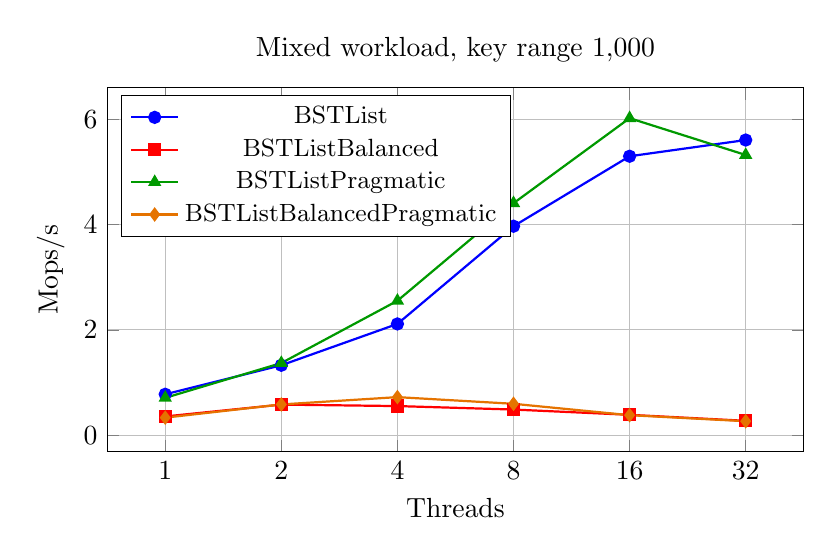
\begin{tikzpicture}
\begin{axis}[
  width=0.86\textwidth,
  height=6.2cm,
  xlabel={Threads},
  ylabel={Mops/s},
  xmode=log,
  log basis x=2,
  xtick={1,2,4,8,16,32},
  xticklabels={1,2,4,8,16,32},
  grid=major,
  legend style={font=\small,at={(0.02,0.98)},anchor=north west},
  title={Mixed workload, key range 1,000}
]
\addplot[color=blue, mark=*, thick] coordinates {(1,0.777)(2,1.328)(4,2.113)(8,3.969)(16,5.298)(32,5.606)};
\addplot[color=red, mark=square*, thick] coordinates {(1,0.356)(2,0.581)(4,0.553)(8,0.487)(16,0.387)(32,0.273)};
\addplot[color=green!60!black, mark=triangle*, thick] coordinates {(1,0.709)(2,1.370)(4,2.553)(8,4.406)(16,6.021)(32,5.322)};
\addplot[color=orange!90!black, mark=diamond*, thick] coordinates {(1,0.333)(2,0.584)(4,0.723)(8,0.596)(16,0.380)(32,0.265)};
\legend{BSTList,BSTListBalanced,BSTListPragmatic,BSTListBalancedPragmatic}
\end{axis}
\end{tikzpicture}
\caption{Mixed throughput at key range 1,000. The store-based unbalanced variant leads from 2 to 16 threads; the barrier-based variant is fastest at 1 and 32 threads.}
\label{fig:mixed-1k}
\end{figure}

The unbalanced variants consistently outperform the balanced variants at all key ranges. The balanced index pays LLX/SCX synchronization and rebalancing overhead on every update, which dominates the small traversal saving it provides. At key range 1,000, the store-based unbalanced variant leads from 2 to 16 threads. The barrier-based variant is marginally faster at 1 thread and at 32 threads (5.606 versus 5.322 Mops/s). Under high contention the plain-store repairs of the pragmatic variant leave backward pointers more frequently stale, causing more retries from head; additionally, each store-based repair now retires the displaced \code{PrevWrapper} through DEBRA, adding a small per-call overhead that accumulates at high thread counts. At the larger key ranges (10,000 and 100,000), forward list traversal dominates the total cost, so the two unbalanced variants are close throughout. At key range 10,000 they alternate as the narrow leader across thread counts; the differences are within measurement noise and should not be over-interpreted.

\subsection{Comparison with a blocking baseline}

\Cref{tab:locked-comparison} compares the two strongest lock-free variants with \code{LockedSet}, a coarse-grained locked baseline built from \code{std::set} and a single \code{std::mutex}. This baseline is useful because it is simple and supports the full operation set. However, every operation must acquire the same lock, so threads cannot make progress in parallel.

\begin{table}[H]
\centering
\caption{Mixed throughput in Mops/s at key range 1,000: lock-free variants vs.\ coarse-grained locked baseline.}
\label{tab:locked-comparison}
\begin{tabular}{r r r r}
\toprule
Threads & \code{LockedSet} & \code{BSTList} & \code{BSTListPragmatic} \\
\midrule
 1 & \textbf{8.468} & 0.777 & 0.709 \\
 2 & \textbf{2.070} & 1.328 & 1.370 \\
 4 & 1.353 & 2.113 & \textbf{2.553} \\
 8 & 0.912 & 3.969 & \textbf{4.406} \\
16 & 0.663 & 5.298 & \textbf{6.021} \\
\bottomrule
\end{tabular}
\end{table}

At one thread, \code{LockedSet} is much faster because \code{std::set} is a sequential balanced tree and does not pay for atomic operations, helping, or memory reclamation. The lock-free variants have higher single-thread overhead because they use compare-and-swap operations, tagged pointers, and DEBRA critical sections even when there is no contention.

The crossover occurs between two and four threads. Once several threads compete for the same mutex, \code{LockedSet} serializes the workload and its throughput drops. In contrast, the lock-free variants allow several operations to make progress at the same time. At 16 threads, \code{BSTListPragmatic} is over 9$\times$ faster than \code{LockedSet}.

\subsection{Comparison with a lock-free balanced tree}
\label{sec:cbat-comparison}

\Cref{tab:cbat-comparison} compares the two unbalanced BST+List variants with CBAT~\cite{wrench2026cbat}. CBAT is a lock-free balanced chromatic tree with augmentation support. It supports \code{insert}, \code{remove}, \code{min}, and \code{max}, but it does not support \code{extract\_min} or \code{extract\_max}. Therefore, this comparison uses the same 40\% \code{insert} / 40\% \code{remove} / 20\% \code{min}+\code{max} workload. Destructive extrema operations (\code{extract\_min}, \code{extract\_max}) are excluded because CBAT does not support them.

\begin{table}[H]
\centering
\caption{Mixed throughput in Mops/s: lock-free BST+List variants vs.\ CBAT.}
\label{tab:cbat-comparison}
\begin{tabular}{r r r r r r r}
\toprule
 & \multicolumn{3}{c}{Key range 1,000} & \multicolumn{3}{c}{Key range 10,000} \\
\cmidrule(lr){2-4}\cmidrule(lr){5-7}
Threads & \code{BSTList} & \code{BSTListPragmatic} & \code{CBAT} & \code{BSTList} & \code{BSTListPragmatic} & \code{CBAT} \\
\midrule
 1 & 0.676 & \textbf{0.766} & 0.127 & 0.037 & 0.040 & \textbf{0.127} \\
 2 & 1.129 & \textbf{1.354} & 0.261 & 0.055 & 0.059 & \textbf{0.191} \\
 4 & 2.363 & \textbf{2.520} & 0.424 & 0.092 & 0.097 & \textbf{0.303} \\
 8 & 3.810 & \textbf{4.514} & 0.632 & 0.162 & 0.169 & \textbf{0.540} \\
16 & \textbf{5.317} & 4.985 & 1.059 & 0.288 & 0.285 & \textbf{0.926} \\
\bottomrule
\end{tabular}
\end{table}

At one thread, CBAT shows similar throughput (approximately 0.127 Mops/s) at both key ranges. This is consistent with CBAT's per-operation constant overhead — descriptor allocation, LLX/SCX synchronization — dominating log(n) tree-height cost at these scales. The tree is roughly 10--13 levels tall across both key ranges, so the height difference contributes a modest fraction of the total per-operation time.

The results depend strongly on the key range. At key range 1,000, the BST+List variants are faster than CBAT at every thread count. The list is short enough that traversal is relatively cheap, so the fixed overhead of CBAT's LLX/SCX synchronization and chromatic-tree rebalancing is more visible. At 16 threads the barrier-based variant (5.317 Mops/s) marginally leads the store-based variant (4.985 Mops/s); this reversal mirrors the pattern in the main mixed table and is explained by the same mechanism: under sustained high contention, the pragmatic variant's \code{PrevWrapper} retirement adds up across many concurrent operations.

At key range 10,000, the result reverses. CBAT is faster because update operations in the BST+List design require two stages: first, a traversal of the hint tree to find a nearby list node, and second, a traversal of the linked list to validate the exact position. CBAT performs a single balanced-tree traversal and then applies the update directly in the tree. Both implementations use DEBRA for memory reclamation (CBAT is compiled with \texttt{-DDEBRA\_ORIGINAL\_FREE}), so reclamation overhead is comparable and does not explain the throughput difference.

The \code{min} and \code{max} operations are not the main bottleneck in this comparison. In the BST+List design, \code{min} starts near \code{head} and \code{max} starts from the backward hint near \code{tail}, so both are efficient in steady state. The limiting factor at larger key ranges is the cost of \code{insert} and \code{remove}, where the list traversal after the hint lookup becomes expensive.

This also explains why the balanced-hint variants in \cref{tab:mixed-throughput} do not close the gap with CBAT. They pay the cost of a chromatic-tree lookup, but they still have to traverse and validate the linked list afterward. In CBAT, the balanced tree is the data structure itself. In this project, the balanced tree is only a hint, so its cost is added on top of the list traversal rather than replacing it.

This comparison should therefore be read carefully. CBAT is a strong baseline for workloads with \code{insert}, \code{remove}, \code{min}, and \code{max}. It is not a complete baseline for this project because it does not support \code{extract\_min} or \code{extract\_max}, those operations are specific to the BST+List design in this evaluation, as discussed in \cref{sec:eval-baselines}.

\subsection{Per-operation results}

\Cref{tab:per-operation} isolates the main operation types at 8 threads and key range 10,000. The results show that the unbalanced variants are better for ordinary updates. \code{BSTListPragmatic} leads for \code{extract\_min} at 1.396 Mops/s, while \code{BSTList} leads for \code{extract\_max} at 1.602 Mops/s.

The \code{extract\_max} result now favours the barrier variant. Although store-based backward-pointer repair is cheaper per call, \code{extract\_max} issues multiple \code{store\_prev\_direct} calls per extraction, and each call now retires the displaced \code{PrevWrapper} through DEBRA. The resulting retirement volume outweighs the per-call simplicity advantage. For \code{extract\_min}, the epoch-based protocol issues fewer backward-pointer writes, so \code{BSTListPragmatic} retains its edge there. The balanced variants remain slower for destructive operations because the balanced hint index adds LLX/SCX and rebalancing overhead.

The \code{min}+\code{max} result is more sensitive to run-to-run variation, because these operations are short and are strongly affected by cache and memory-bandwidth behavior on the shared server. The unusually high value for \code{BSTListBalancedPragmatic} should therefore be interpreted with caution unless it is confirmed by repeated runs.

\begin{table}[H]
\centering
\caption{Per-operation throughput in Mops/s, 8 threads, key range 10,000.}
\label{tab:per-operation}
\begin{tabular}{l r r r r r}
\toprule
Variant & insert & remove & min+max & extract\_min & extract\_max \\
\midrule
\code{BSTList} & \textbf{0.053} & \textbf{0.050} & 24.972 & 1.367 & \textbf{1.602} \\
\code{BSTListBalanced} & 0.038 & 0.024 & 25.721 & 0.227 & 0.225 \\
\code{BSTListPragmatic} & 0.043 & 0.032 & 26.429 & \textbf{1.396} & 1.064 \\
\code{BSTListBalancedPragmatic} & 0.038 & 0.023 & \textbf{27.974} & 0.239 & 0.253 \\
\bottomrule
\end{tabular}
\end{table}

\begin{figure}[H]
\centering
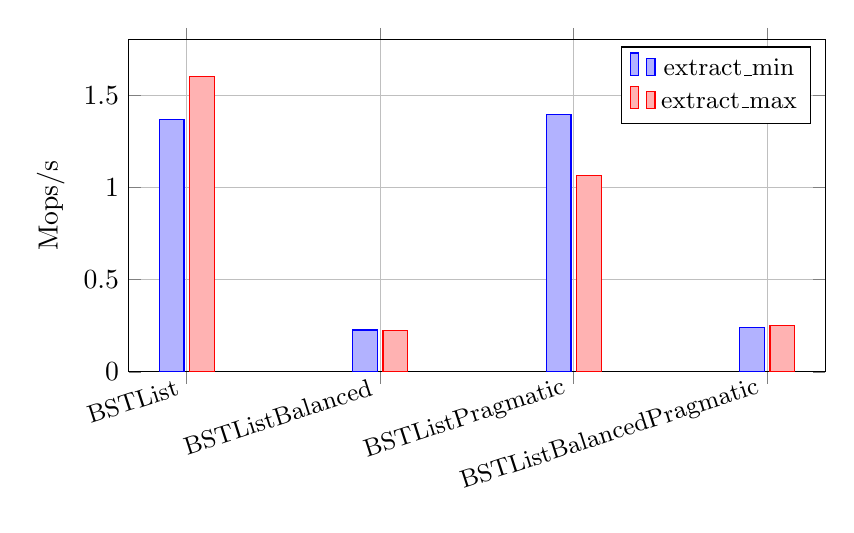
\begin{tikzpicture}
\begin{axis}[
  ybar,
  width=0.86\textwidth,
  height=5.8cm,
  bar width=9pt,
  ylabel={Mops/s},
  symbolic x coords={BSTList,BSTListBalanced,BSTListPragmatic,BSTListBalancedPragmatic},
  xtick=data,
  xticklabel style={rotate=18,anchor=east,font=\small},
  legend style={font=\small,at={(0.98,0.98)},anchor=north east},
  ymin=0,
  ymax=1.8,
  grid=major
]
\addplot coordinates {(BSTList,1.367)(BSTListBalanced,0.227)(BSTListPragmatic,1.396)(BSTListBalancedPragmatic,0.239)};
\addplot coordinates {(BSTList,1.602)(BSTListBalanced,0.225)(BSTListPragmatic,1.064)(BSTListBalancedPragmatic,0.253)};
\legend{extract\_min,extract\_max}
\end{axis}
\end{tikzpicture}
\caption{Extract throughput at 8 threads and key range 10,000.}
\label{fig:extract-throughput}
\end{figure}

\section{Discussion}

The experiments suggest three main conclusions.

First, the store-based list is usually the stronger list backend for mid-range thread counts. Replacing compare-and-swap repairs of backward pointers with direct atomic exchanges reduces per-call synchronization overhead. This benefit is clearest for \code{max} and \code{extract\_min}, where fewer backward-pointer writes are issued per operation. For \code{extract\_max}, however, each extraction issues several backward-pointer updates and each one now retires a displaced \code{PrevWrapper} through DEBRA; this retirement volume reverses the advantage, and the barrier variant leads for that operation.

Second, the balanced hint index did not help in these workloads. A chromatic tree gives better worst-case height than an unbalanced BST, but it also adds LLX/SCX synchronization and rebalancing. Since the tree is only a hint, the operation still has to validate its result in the list. In the measured workloads, the extra tree cost was larger than the traversal time saved by the better hint.

Third, the design is most effective when the list is not too large or when the workload contains many extrema operations. At larger key ranges, \code{insert} and \code{remove} spend more time traversing the list after receiving a hint. This is the main tradeoff of keeping correctness in the list and using the tree only as an auxiliary hint structure.

One notable exception is the 32-thread result at key range 1,000, where the barrier variant is slightly faster than the pragmatic variant (5.606 versus 5.322 Mops/s). At this thread count the list is short and contention is very high. The plain stores used by the pragmatic variant allow backward pointers to become stale more quickly under sustained concurrent pressure, which forces more retries from head. The barrier variant's compare-and-swap repairs maintain fresher backward pointers and reduce those retries enough to recover the small overhead difference. The same dynamic is visible at 1 thread: there the barrier variant (0.777 Mops/s) is marginally ahead of the pragmatic variant (0.709 Mops/s), likely because the added DEBRA retirement in each \code{store\_prev\_direct} call is a measurable overhead when the workload has very low parallelism and the benefit of avoiding CAS loops is small.

A related consequence is that the advantage of the store-based backend becomes smaller at larger key ranges. The pragmatic variant mainly helps by making backward-pointer maintenance cheaper. At key range 100,000, the forward traversal in \code{insert} and \code{remove} dominates total running time, so the cost of \code{prev} repair matters less. As a result, the two unbalanced variants are essentially equal in the 100,000 key-range rows of \cref{tab:mixed-throughput}, with neither consistently ahead.

\section{Limitations and Future Work}

The current implementation has several limitations. The BST hint index is only approximately maintained, and the measured hint quality is not strong enough to remove long list traversals at large key ranges. The balanced hint index also has high overhead because it performs full chromatic-tree rebalancing even though the list, not the tree, defines correctness.

Future work should focus on improving the data structure rather than only improving the benchmarks. Several directions look promising.

\paragraph{A cheaper balanced hint structure.}
A full lock-free chromatic tree may be more powerful than needed for a hint index. A future version could use a cheaper approximate index, such as a relaxed skip-list hint, a sampled index, or a partially rebuilt tree. Since the index is only a hint, it may not need to rebalance after every update.

\paragraph{Reducing wrapper allocation overhead.}
The pragmatic variant now uses \code{atomic\_exchange} for \code{prev} repairs, which allows the displaced \code{PrevWrapper} to be retired immediately through DEBRA. The remaining overhead is the allocation of a new wrapper on every repair. A future version could reduce this cost using a pool allocator, or by using a tagged integer representation for \code{prev} that avoids heap allocation entirely.

\paragraph{More precise memory ordering.}
The implementation could be reviewed to use the weakest correct memory orders. For example, advisory backward-pointer stores may not need the same ordering as correctness-critical forward-pointer compare-and-swap operations. Reducing unnecessary acquire-release synchronization could improve performance, especially on multi-socket machines.

\paragraph{Adaptive back-pointer repair.}
The current implementations choose one repair strategy globally. A future implementation could adapt: use plain stores under low risk, use compare-and-swap repairs when backward links become too stale, and use bounded cleanup near \code{tail} when \code{max} or \code{extract\_max} detects poor hint quality.

\paragraph{NUMA-aware allocation and reclamation.}
The benchmarks run on a multi-socket server. Allocating list nodes and retirement bags with NUMA awareness may reduce cross-socket memory traffic. This is especially relevant because the list and DEBRA structures are accessed by many threads.

\section{Conclusion}

This project implemented and evaluated a lock-free ordered list with BST hints. The central design choice is to keep correctness in the list and use the tree only to find good starting points for traversal. This makes stale tree entries safe and allows different hint indexes to be used without changing the list-level correctness argument.

The store-based unbalanced variant is the strongest variant at most thread counts, and leads for \code{extract\_min}. The barrier-based variant leads for \code{extract\_max}, where the retirement cost of each backward-pointer update outweighs the CAS savings. The balanced hint index did not improve throughput in the tested configurations, which suggests that a hint structure should be much cheaper than a full balanced lock-free tree. The comparison with CBAT also shows the main tradeoff: a true balanced tree is better for large update-heavy workloads, while the BST+List design provides efficient destructive extrema operations that CBAT does not support.

\section*{Declaration of AI Use}

Claude Code was used as an AI coding assistant during the project. It helped generate code skeletons, translate pseudocode into C++, identify possible bugs, and draft preliminary text. The algorithmic choices, correctness reasoning, experiments, and final report were reviewed and edited by the author.

\bibliographystyle{plain}
\begin{thebibliography}{10}

\bibitem{brown2015debra}
Trevor Brown.
\newblock Reclaiming memory for lock-free data structures: There has to be a better way.
\newblock In \emph{Proceedings of the 2015 ACM Symposium on Principles of Distributed Computing}, pages 261--270, 2015.

\bibitem{brown2014general}
Trevor Brown, Faith Ellen, and Eric Ruppert.
\newblock A general technique for non-blocking trees.
\newblock In \emph{Proceedings of the 19th ACM SIGPLAN Symposium on Principles and Practice of Parallel Programming}, pages 329--342, 2014.

\bibitem{fomitchev2004lock}
Mikhail Fomitchev and Eric Ruppert.
\newblock Lock-free linked lists and skip lists.
\newblock In \emph{Proceedings of the 23rd Annual ACM Symposium on Principles of Distributed Computing}, pages 50--59, 2004.

\bibitem{harris2001pragmatic}
Timothy L. Harris.
\newblock A pragmatic implementation of non-blocking linked-lists.
\newblock In \emph{Proceedings of the 15th International Symposium on Distributed Computing}, pages 300--314, 2001.

\bibitem{melnikov2024hinted}
Vladimir Melnikov and Gal Sela.
\newblock Concurrent extrema and successor/predecessor queries in search trees.
\newblock Semester project report, EPFL/Technion, 2026.

\bibitem{natarajan2014fast}
Aravind Natarajan and Neeraj Mittal.
\newblock Fast concurrent lock-free binary search trees.
\newblock In \emph{Proceedings of the 19th ACM SIGPLAN Symposium on Principles and Practice of Parallel Programming}, pages 317--328, 2014.

\bibitem{traff2020pragmatic}
Jesper Larsson Tr\"{a}ff and Martin P\"{o}ter.
\newblock A more pragmatic implementation of the lock-free, ordered, linked list.
\newblock arXiv:2010.15755, 2020.

\bibitem{brown2020setbench}
Trevor Brown.
\newblock SetBench: A benchmark suite and code library for concurrent sets and maps.
\newblock \url{https://gitlab.com/trbot86/setbench}, 2020.

\bibitem{wrench2026cbat}
Evan Wrench, Ajay Singh, Younghun Roh, Panagiota Fatourou, Siddhartha Jayanti, Eric Ruppert, and Yuanhao Wei.
\newblock Concurrent balanced augmented trees.
\newblock In \emph{Proceedings of the 31st ACM SIGPLAN Annual Symposium on Principles and Practice of Parallel Programming}, 2026.

\end{thebibliography}

\end{document}
